%% astroARIADNE II -- working draft (A&A)
%%
%% Built from ariadne_II_skeleton.tex (2026-08-07), which is kept unchanged as the
%% record of that session. Numbers in the tables are MEASURED and traceable to
%% scripts in IRX_experiment/injection_recovery/.
%% 2026-11-23: every calibration number now comes from the final run cal_run4
%% (4158 injections, 1367 survey stars, 169 roster stars; code 71d4470, Sonora
%% companion injections, covariant error budget) through
%% cal_run4_analysis/run.sh -> paper_numbers.py, which writes
%% ariadne_II_numbers.tex (macros) and tab_inj/tab_bycat/tab_calib.tex (table
%% bodies). The cal_run2 provenance below is superseded and kept as record:
%%     roster_cal2_res/   roster refit with the final code (fit_real_one.py on
%%                        roster_frozen_irsfix/, stitched IRS); analyze_roster_ab.py F
%%     cal_run2/          injections (res_inj) + survey (res_real), final code;
%%                        table1_injections.py --cal, build_pool_cal.py,
%%                        uvw_banyan.py, crossmatch_disks.py, build_candidate_table.py
%%                        (all via post_cal.sh), survey_stats_cal.py
%%     baseline_nulls/    mid-IR baseline calibration (246 field dwarfs)
%%     refreeze_irs_stitch.py, refreeze_hosts_irs.py   stitched IRS photometry
%% Method text (Sect. 3) is written against astroARIADNE/fitter.py on branch v2
%% (_compute_irx, _excess_model_selection, fit_irx) as of 0900b88.
%% Anything not verified is marked \todo{} rather than guessed.
%%
%% Scope (Jose, 2026-08-19): this is a DISK paper framed on the disk-vs-companion
%% degeneracy. The JWST/MIRI programme is not its resolution and is not
%% mentioned as one.

\documentclass{aa}
\usepackage{graphicx}
\usepackage{amsmath}
\usepackage{booktabs}
\usepackage{txfonts}
\usepackage[colorlinks,citecolor=blue]{hyperref}
\newcommand{\todo}[1]{\textcolor{red}{[TODO: #1]}}
\newcommand{\ariadne}{\texttt{astroARIADNE}}
\newcommand{\nirx}{n_{\mathrm{IRX}}}
\newcommand{\Lsun}{L_\odot}
\newcommand{\Rsun}{R_\odot}
%% Generated by IRX_experiment/injection_recovery/cal_run4_analysis/paper_numbers.py
%% from the cal_run4 analysis outputs (run4/numbers_*.json). Do not edit by hand.
\newcommand{\nInj}{4158}
\newcommand{\nInjDisk}{2058}
\newcommand{\nInjComp}{2100}
\newcommand{\nInjHosts}{seven}
\newcommand{\injTdMin}{100}
\newcommand{\injTdMax}{1100}
\newcommand{\injFdMin}{3\times10^{-5}}
\newcommand{\injFdMax}{1\times10^{-2}}
\newcommand{\injTtwoMin}{700}
\newcommand{\injTtwoMax}{2600}
\newcommand{\injRtwoMin}{0.07}
\newcommand{\injRtwoMax}{0.16}
\newcommand{\injAtmoTmin}{2600}
\newcommand{\injDiskAllPct}{51.4}
\newcommand{\injDiskAllN}{2058}
\newcommand{\injDiskDetectablePct}{78.1}
\newcommand{\injDiskDetectableN}{1176}
\newcommand{\injDiskDeclaredPct}{97.2}
\newcommand{\injDiskDeclaredN}{788}
\newcommand{\injDiskFlagPct}{38.3}
\newcommand{\injDiskFlagPctInt}{38}
\newcommand{\injCompAllPct}{30.7}
\newcommand{\injCompAllN}{2100}
\newcommand{\injCompDetectablePct}{34.2}
\newcommand{\injCompDetectableN}{798}
\newcommand{\injCompDeclaredPct}{100.0}
\newcommand{\injCompDeclaredN}{50}
\newcommand{\injCompFlagPct}{2.4}
\newcommand{\injCompFlagPctInt}{2}
\newcommand{\injCompOneIn}{42}
\newcommand{\injCompAsDiskAllPct}{4.1}
\newcommand{\injCompAsDiskDet}{no}
\newcommand{\injDiskAsCompDet}{12}
\newcommand{\injDiskDet}{788}
\newcommand{\injCompDet}{50}
\newcommand{\injCompDetSco}{0}
\newcommand{\injCompNSco}{315}
\newcommand{\injCompDetGJ}{0}
\newcommand{\injCompNGJ}{315}
\newcommand{\injCompDetLHS}{19}
\newcommand{\injCompNLHS}{280}
\newcommand{\injCompDetLal}{0}
\newcommand{\injCompNLal}{315}
\newcommand{\injCompDetProx}{0}
\newcommand{\injCompNProx}{315}
\newcommand{\injCompDetVB}{31}
\newcommand{\injCompNVB}{245}
\newcommand{\injCompDetDra}{0}
\newcommand{\injCompNDra}{315}
\newcommand{\injCompNoDetHostsN}{1575}
\newcommand{\injCompDetHosts}{two}
\newcommand{\injVBcoolTmax}{400}
\newcommand{\injVBcoolN}{63}
\newcommand{\injVBcoolOK}{63}
\newcommand{\injVBwarmT}{600}
\newcommand{\injVBwarmN}{seven}
\newcommand{\injVBwarmOK}{two}
\newcommand{\injVBwarmComp}{no}
\newcommand{\injVBwarmAmb}{five}
\newcommand{\injDetLHS}{82}
\newcommand{\injDetOKLHS}{82}
\newcommand{\injDetCompLHS}{0}
\newcommand{\injDetProx}{55}
\newcommand{\injDetOKProx}{54}
\newcommand{\injDetCompProx}{0}
\newcommand{\injDetGJ}{106}
\newcommand{\injDetOKGJ}{92}
\newcommand{\injDetCompGJ}{12}
\newcommand{\injGJcoldComp}{seven}
\newcommand{\injGJcoldTmin}{100}
\newcommand{\injGJcoldTmax}{175}
\newcommand{\injGJwarmComp}{five}
\newcommand{\injGJwarmTmin}{600}
\newcommand{\injGJwarmTmax}{850}
\newcommand{\injGJTtwoMin}{2271}
\newcommand{\injGJTtwoMax}{3155}
\newcommand{\injGJRtwoMin}{0.23}
\newcommand{\injGJRtwoMax}{0.39}
\newcommand{\injGJcoldNsig}{two}
\newcommand{\nRoster}{169}
\newcommand{\rosSkipped}{Seventeen}
\newcommand{\rosNoTruth}{fourteen}
\newcommand{\rosFitFail}{three}
\newcommand{\rosDC}{61}
\newcommand{\rosDCok}{59}
\newcommand{\rosDCweak}{one}
\newcommand{\rosDCinf}{18}
\newcommand{\rosDClnbMed}{136}
\newcommand{\rosDClnbMin}{2.3}
\newcommand{\rosNondetLnbMed}{0.4}
\newcommand{\rosDCwrong}{two}
\newcommand{\ppLnbMin}{60}
\newcommand{\ppLnbMax}{142}
\newcommand{\ppFdMin}{0.02}
\newcommand{\ppFdMax}{0.06}
\newcommand{\ppNq}{three}
\newcommand{\ppJzzNsig}{no}
\newcommand{\contamDet}{eight}
\newcommand{\contamDisk}{eight}
\newcommand{\contamLnbMin}{2.8}
\newcommand{\contamLnbMax}{725}
\newcommand{\ophLnb}{-5.8}
\newcommand{\twaTd}{76}
\newcommand{\twaFd}{1.3\times10^{-3}}
\newcommand{\gjFiveNsig}{two}
\newcommand{\glOneTtwo}{3450}
\newcommand{\glOneRtwo}{0.24}
\newcommand{\glOneTeff}{3500}
\newcommand{\wdDiskOK}{11}
\newcommand{\wdDiskN}{27}
\newcommand{\wdCompOK}{one}
\newcommand{\wdCompN}{18}
\newcommand{\relN}{104}
\newcommand{\relOverconf}{+0.070}
\newcommand{\relBrier}{0.399}
\newcommand{\relSatWrongPct}{12}
\newcommand{\svFrozen}{1367}
\newcommand{\svOK}{1349}
\newcommand{\svFewBands}{18}
\newcommand{\svDet}{503}
\newcommand{\svDetDisk}{449}
\newcommand{\svPool}{375}
\newcommand{\svPoolOther}{370}
\newcommand{\svPoolKnown}{Five}
\newcommand{\svPoolKnownLow}{five}
\newcommand{\svTdKnown}{281}
\newcommand{\svTdOther}{226}
\newcommand{\svFdKnown}{4\times10^{-2}}
\newcommand{\svFdOther}{5\times10^{-2}}
\newcommand{\svKnownLnbMin}{60}
\newcommand{\banCtlN}{747}
\newcommand{\banPoolMem}{121}
\newcommand{\banPoolPct}{32}
\newcommand{\banCtlMem}{28}
\newcommand{\banCtlPct}{4}
\newcommand{\banPoolRvN}{85}
\newcommand{\banCtlRvN}{25}
\newcommand{\banPoolRvPct}{24}
\newcommand{\banCtlRvPct}{4}
\newcommand{\banPoolScoPct}{68}
\newcommand{\banCtlScoPct}{16}
\newcommand{\banPoolOutPct}{10}
\newcommand{\banCtlOutPct}{2}
\newcommand{\banPoolPctTwo}{51}
\newcommand{\banCtlPctTwo}{17}
\newcommand{\banRatio}{nine}
\newcommand{\banLCC}{70}
\newcommand{\banUCL}{17}
\newcommand{\banUSCO}{8}
\newcommand{\banPPhiMin}{0.95}
\newcommand{\banPPhiMax}{0.99}
\newcommand{\banPPlo}{0.78}
\newcommand{\xmMembers}{121}
\newcommand{\xmDiskBearing}{75}
\newcommand{\xmLtwotwo}{70}
\newcommand{\xmKnownPP}{three}
\newcommand{\xmDiskless}{Two}
\newcommand{\xmNew}{41}
\newcommand{\xmNewByGroup}{15 in Lower Centaurus--Crux, 7 in Upper Scorpius, 5 in $\epsilon$\,Cha, 5 in $\chi^1$\,For, and 4 in Upper Centaurus--Lupus}
\newcommand{\accN}{80}
\newcommand{\accKnownPP}{three}
\newcommand{\candA}{27}
\newcommand{\candAnoMem}{23}
\newcommand{\candY}{43}
\newcommand{\candYA}{four}
\newcommand{\candN}{66}
\newcommand{\svWthreeMed}{3.6}
\newcommand{\svWthreeMin}{0.46}
\newcommand{\svLowBPct}{57}
\newcommand{\svHighB}{41}
\newcommand{\svNeos}{139}


\begin{document}

\title{astroARIADNE II: infrared-excess model selection in Bayesian
       model-averaged SED fitting, and the limits of archival
       classification\thanks{{\it Herschel} is an ESA space observatory with
       science instruments provided by European-led Principal Investigator
       consortia and with important participation from NASA.}}

\titlerunning{astroARIADNE II: infrared-excess model selection}
\author{J. I. Vines\inst{1}}
\authorrunning{J. I. Vines}
\institute{Instituto de Astronom\'ia, Universidad Cat\'olica del Norte,
           Angamos 0610, Antofagasta, Chile}

\abstract
% context
{An infrared excess may arise from circumstellar dust, an unresolved cool
companion, or an unrelated source in a large photometric beam. Telling them apart
matters for debris-disk statistics and for vetting exoplanet hosts.}
% aims
{We extend \ariadne{} with Bayesian model selection over four infrared-excess
hypotheses and determine where archival broadband photometry can support a
classification.}
% methods
{The excess is measured against the model-averaged photosphere, on bands that
every grid in the ensemble reaches. The evidence for no excess, a
single- or two-temperature dust component, and a substellar companion is computed
by direct quadrature over physical priors, the companion averaged over five cool
atmosphere grids. We validate it with \nInj{} injections and \nRoster{} stars of known
nature.}
% results
{Once an excess is detected, dust and companions separate: \rosDCok{} of the \rosDC{} roster
stars with a detected excess of known origin are assigned their true class,
decisively, and no detected injected companion is taken for dust. The
physical priors do the work: a companion no larger than its primary cannot supply
a cold, luminous excess. The degeneracy survives only for warm dust
around the coolest hosts. Archival classification is limited instead by
sensitivity (\injDiskFlagPctInt\% of injected disks and \injCompFlagPct\% of injected companions are
detected), by flux from unrelated sources, which is classified as dust, by a
second stellar photosphere that the joint fit of a cool host can substitute for a
weak excess, and by
probabilities that saturate for two thirds of stars. Among 1372 nearby M dwarfs the method recovers the known
Peter Pan disks, together with \svPoolOther{} stars it cannot tell apart from them; \banPoolPct\% of
these belong to young associations, mostly in Sco-Cen, against \banCtlPct\% of matched
stars without an excess, and \candN{} are new disk candidates.}
% conclusions
{A broadband SED can decide whether an excess is dust or a companion. It cannot
decide whether the excess belongs to the star.}

\keywords{stars: fundamental parameters -- circumstellar matter --
          infrared: stars -- methods: statistical -- binaries: close}

\maketitle

%%%%%%%%%%%%%%%%%%%%%%%%%%%%%%%%%%%%%%%%%%%%%%%%%%%%%%%%%%%%%%%%%%%%%%%%%%%%%%%
\section{Introduction}
\label{sec:intro}

Emission in excess of the stellar photosphere at mid- and far-infrared wavelengths
is the principal tracer of circumstellar dust, from primordial and accretion disks
to the debris disks that outlive them
\citep{wyatt2008,hughes2018}. All-sky surveys, WISE above all
\citep{wright2010}, have turned the search for such excesses into a catalogue
exercise, and several large samples of infrared-excess stars now exist
\citep[e.g.][]{patel2014,cotten2016,mcdonald2017}.

An excess, however, is not diagnostic of dust. Any source that is unresolved from
the star and cooler than it adds flux at long wavelengths: a low-mass stellar or
substellar companion, or an unrelated background object inside the
$6\farcs5$--$12\arcsec$ beam of WISE W3 and W4. For faint targets the background
term dominates \citep{kennedy2012}. M-dwarf excesses are particularly exposed:
all thirteen of the \citet{theissen2014} candidates bright enough in W4 to be
inspected were found to be extended or multiple in the WISE images and rejected
by \citet{silverberg2018}, and several of the W3/W4-selected M dwarfs of
\citet{ren2026} show evidence of background contamination. Around white dwarfs the disk and
companion interpretations are degenerate in broadband photometry, and separating
them has required near-infrared spectroscopy \citep{owens2023}. Recent surveys
state the same ambiguity for field stars \citep{esteves2026}.

The tools used to find excesses do not, in general, weigh these alternatives
against each other. The usual procedure fits a photosphere, flags bands whose
residual exceeds a significance or colour threshold, and characterises the excess
with a single blackbody
\citep[e.g.][]{bayo2008,mcdonald2017,mcdonald2024}. A companion, when it is
considered, is treated in a separate analysis. What is missing is a comparison of
the competing hypotheses on the same data, by the same statistic, with the
uncertainty in the photosphere carried through to the excess.

\ariadne{} \citep{vines2022} already has the ingredients for that comparison. It
fits a star's photometry with several model-atmosphere grids and combines them by
Bayesian model averaging \citep{hoeting1999}, weighting each grid by its evidence,
so that the spread between grids enters the stellar parameters. It remains the
only published SED fitter to average over atmosphere grids rather than select one
\citep[cf.][]{andrae2023,mcdonald2024}. The same machinery extends naturally to
the excess: the model-averaged photosphere, together with its grid-to-grid
scatter, is the baseline against which an excess is measured, and the hypotheses
for that excess can be compared by their evidence, exactly as the grids are.

In this paper we add that comparison to \ariadne{}, over four hypotheses: no
excess, a single-temperature dust component, a two-temperature dust component, and
a substellar companion (Sect.~\ref{sec:method}). The larger part of the paper then
measures where the comparison can be trusted. We validate it with \nInj{}
injection--recovery tests and a literature roster of stars whose nature is known
(Sect.~\ref{sec:validation}), show that dust and companions separate whenever an
excess is detected and explain why (Sect.~\ref{sec:separate}), identify what
limits archival classification instead (Sect.~\ref{sec:fail}), and apply the
method to 1372 nearby M dwarfs to establish what an archival search for
long-lived M-dwarf disks can and cannot deliver (Sect.~\ref{sec:survey}).


%%%%%%%%%%%%%%%%%%%%%%%%%%%%%%%%%%%%%%%%%%%%%%%%%%%%%%%%%%%%%%%%%%%%%%%%%%%%%%%
\section{Method}
\label{sec:method}

\subsection{The photosphere and the excess}
\label{sec:excess}

The photosphere is fitted as in \citet{vines2022}: each grid in the ensemble is
sampled with \texttt{dynesty} \citep{speagle2020}, and the posteriors are averaged
with weights proportional to the grids' evidences. Only bands blueward of a cut
wavelength $\lambda_{\rm cut}$ enter this fit; bands redward of it are withheld
and form the excess set (Sect.~\ref{sec:bandset}).

For each excess band $b$ we draw 256 samples from the model-averaged posterior,
choosing a grid according to its weight and a parameter vector from that grid's
posterior, and evaluate the synthetic flux. The mean of these draws is the
predicted photospheric flux $F^\star_b$. The grid evidences are set by the optical
and near-infrared fit bands and say nothing about how well each grid's physics
holds at $10$--$500\,\mu$m, so the between-grid part of the photospheric
uncertainty $\sigma^\star_b$ is the equal-weight spread of the grids' mean
predictions about $F^\star_b$; the within-grid part keeps the evidence weights, and
$\sigma^\star_b$ is never smaller than the standard deviation of the draws. The
excess and its uncertainty are
\begin{equation}
  \begin{aligned}
  \Delta F_b &= F^{\rm obs}_b - F^\star_b , \\
  \sigma_b^2 &= \left(\sigma^{\rm obs}_b\right)^2 + \left(c_b\,F^{\rm obs}_b\right)^2
             + \sigma_{{\rm conf},b}^2 + \left(\sigma^\star_b\right)^2 ,
  \end{aligned}
  \label{eq:excess}
\end{equation}
where $c_b$ is the absolute calibration uncertainty of the instrument that
measured band $b$, which catalogue errors omit: 2.4, 2.8, 4.5 and 5.7\% for W1--W4
\citep{jarrett2011}; 3\% for IRAC and 5\% for the IRS bands; 2, 5 and 12\% for
MIPS; 3 and 4\% for AKARI/IRC \citep{ishihara2010} and 20--40\% for AKARI/FIS;
3.6--10.4\% for IRAS; 5\% for PACS and 4.3\% for SPIRE; 1.4 and 2.2\% for SPHEREx
below and above $3.82\,\mu$m; and 2\% for any other band \todo{cite the IRAC, MIPS, IRS, PACS, SPIRE, IRAS, FIS and
SPHEREx calibration references listed in docs/irx.md}. Bands of one instrument
share its absolute scale, so $c_b$ is split into a term common to the instrument's
bands and an independent term; where the source does not document the split, the
smallest $c_b$ of the instrument is taken as common. Two bands $b \ne b'$ of one
instrument then have covariance $a_b a_{b'} F^{\rm obs}_b F^{\rm obs}_{b'}$, with
$a_b$ the common term, and the excess residuals enter every hypothesis through
the full covariance matrix $\mathsf{C}$. Its determinant does not depend on the
hypothesis and cancels from the evidence ratios. $\sigma_{{\rm conf},b}$ is the extragalactic confusion
noise of the far-infrared bands: 5.8, 6.3 and 6.8\,mJy for SPIRE
\citep{nguyen2010}, 0.15 and 0.68\,mJy for PACS at 100 and $160\,\mu$m
\citep{magnelli2013}, and 0.64 and 8\,mJy for MIPS at 70 and $160\,\mu$m, the
$5\sigma$ limits of \citet{dole2004} divided by five. PACS at $70\,\mu$m has no
measured confusion noise at any published depth \citep{berta2011} and is given
none. It is zero shortward of $70\,\mu$m. The significance of the
excess in band $b$ is $s_b = \Delta F_b/\sigma_b$, from the marginal error.

The model photospheres over-predict the mid-infrared flux of M dwarfs by about
10\% (Sect.~\ref{sec:caveats}). We correct the predicted W2, W3 and W4 fluxes by
an empirical factor $1 + r_b(T_{\rm eff})$, the median residual of 246 field
dwarfs without an excess binned in fitted temperature, and add its uncertainty to
$\sigma^\star_b$. The correction is applied only inside the domain in which it was
measured: the WISE bands themselves, $T_{\rm eff} \le 7500$\,K, and magnitudes
fainter than $W2 = 7$, $W3 = 5$ and $W4 = 4.5$, below which saturation biases the
photometry. Calibrated on one random half of the sample and tested on the other,
it brings the median W3 residual of M dwarfs from $-10.0\%$ to $-0.1 \pm 0.9\%$.

Spitzer IRS low-resolution spectra from CASSIS \citep{lebouteiller2011} are binned into eleven top-hat
bands between 5.5 and $35\,\mu$m, each inside a single spectral order. The
short-low slit is 3\farcs6 wide against 10\farcs5 for long-low, so a pointing
offset removes flux from the short-low spectrum alone and leaves a step at the
$14\,\mu$m order seam. We extrapolate each side to the seam with a power law
fitted within its own order, scale the short-low bands to long-low, and add the
fractional size of the correction to their errors. Across the 47 roster spectra
that span the seam the median correction is 9\%; for TWA\,7 it is a factor 3.6
(Sect.~\ref{sec:fail}).

Stars on the white-dwarf sequence of the Gaia colour--magnitude diagram are
fitted with the DA models of \citet{koester2010}, whose spectra end near $3\,\mu$m; beyond that the
photosphere is extrapolated as a Rayleigh--Jeans tail, and $\lambda_{\rm cut}$ is
moved to $1\,\mu$m.

\subsection{Which bands are quantified}
\label{sec:bandset}

An excess is quantified only where it can be measured against a modelled
photosphere rather than an extrapolated one. A grid's reach is the set of
excess bands for which it has finite synthetic fluxes within its native
wavelength coverage. In a model-averaged fit a band is quantified only if it lies
within the reach of \emph{every} grid in the ensemble; bands the star has beyond
that common reach are shown on the SED but carry no model and no excess. To keep
the common reach from collapsing, the ensemble for an excess fit is chosen as
every candidate grid whose reach extends to at least 98\% of the wavelength of the
star's reddest observed excess band, before the temperature gating and
band-coverage checks of the standard fit are applied.

Bands are assigned to the photosphere fit or to the excess set by wavelength
alone. The default $\lambda_{\rm cut} = 4.4\,\mu$m places W2, IRAC\,4.5\,$\mu$m and
the two reddest SPHEREx bands in the excess set together with every band beyond
$5\,\mu$m. W2 is withheld from the fit deliberately. The share of the
system's flux contributed by a 1000--2000\,K companion rises steeply towards W2,
and when W2 is left in the fit the photosphere can absorb the companion's flux.

We call the number of quantified bands $\nirx$. It counts W2 whenever W2 is
observed, so a star with WISE photometry alone has $\nirx = 3$ (W2, W3, W4).

\subsection{Four hypotheses}
\label{sec:hyp}

Each hypothesis $k$ predicts an excess flux $M_{k,b}(\boldsymbol\theta)$ in the
quantified bands $\mathcal{Q}$ and, since an excess component cannot be confined
to long wavelengths, a flux $M_{k,j}(\boldsymbol\theta)$ in the photosphere-fit
bands $\mathcal{F}$ as well. We write
\begin{equation}
  \chi^2_k(\boldsymbol\theta) =
    \mathbf{r}_k^{\sf T}\,\mathsf{C}^{-1}\,\mathbf{r}_k
  + \sum_{j\in\mathcal{F}}
      \frac{M_{k,j}(\boldsymbol\theta)^2}{\tilde\sigma_j^2} ,
  \label{eq:chi2}
\end{equation}
where $r_{k,b} = \Delta F_b - M_{k,b}(\boldsymbol\theta)$ over the quantified
bands, $\mathsf{C}$ is their covariance (Sect.~\ref{sec:excess}), and
$\tilde\sigma_j$ is the photometric error of fit band $j$ inflated by the
noise term fitted for it. The second sum charges each hypothesis for the flux it
would have added to bands the photosphere already fits; without it, a companion
constrained only by W3 and W4 can take temperatures and radii that grossly
overpredict $J$, $H$ and $K_s$.

\paragraph{Null.} $M_{0,b} = 0$, with no free parameters.

\paragraph{Single-temperature dust.} A modified blackbody,
\begin{equation}
  \begin{aligned}
  M_{1,b} &= \Omega\, B_\lambda(T)\,\eta(\lambda), \\
  \eta(\lambda) &= \min\!\left[1,\ (210\,\mu{\rm m}/\lambda)^{\beta}\right],
  \quad \beta = 1 ,
  \end{aligned}
\end{equation}
parametrised by the dust temperature $T$ and the fractional luminosity
\begin{equation}
  f_{\rm d} \equiv \frac{L_{\rm dust}}{L_\star}
  = \frac{4 d^2\, \Omega\, \sigma_{\rm SB} T^4 X(T)}{L_\star},
\end{equation}
where $X(T)$ is the fraction of the blackbody's bolometric flux retained after
the modification. The prior is log-uniform in $T \in [30, 1500]$\,K and in
$f_{\rm d} \in [10^{-7}, 10^{-1}]$, truncated above an empirical ceiling on hot
dust: $f_{\rm max} = 10^{-1}$ at $T \le 500$\,K, falling log-linearly in $T$ to
$10^{-4}$ at 1500\,K, the level of the hot exozodiacal dust observed around
main-sequence stars \citep{kral2017}. Without the ceiling a companion photosphere
can be absorbed by a hot, implausibly luminous blackbody. For white-dwarf hosts,
where hot and comparatively luminous dust is the norm, the ceiling is replaced by
a flat $f_{\rm max} = 10^{-1}$.

\paragraph{Two-temperature dust.} The sum of two such components with
$T_{\rm w} > T_{\rm c}$, the order breaking the labelling degeneracy, and the same
priors and ceiling for each. It is evaluated only when $\nirx \ge 5$.

\paragraph{Substellar companion.} The photosphere of a cool unresolved companion,
$M_{3,b} = R_2^2\,\mathcal{F}_{g,b}(T_2)$, where $\mathcal{F}_{g,b}$ is the flux of
grid $g$ per unit radius, placed at the star's distance and reddened by its
extinction, at $\log g = 5.0$ and the primary's [M/H] (the companion is taken to be
coeval). The prior is uniform in $T_2$ between the grid's lower limit and the
smaller of its upper limit and the primary's $T_{\rm eff}$, and log-uniform in
$R_2$ from $0.03\,\Rsun$ to $R_{2,\rm max}$. For a main-sequence primary
$R_{2,\rm max} = \max(R_1, 0.12\,\Rsun)$: a coeval companion cannot be larger than
its primary, but a degenerate brown dwarf can be larger than a late-M primary, and
the floor keeps such solutions. For a compact primary ($R_1 \le 0.05\,\Rsun$)
$R_{2,\rm max} = 0.15\,\Rsun$, since a companion detected only as an infrared excess
of a white dwarf must be substellar. Solutions with $R_2^2 T_2^4 > R_1^2 T_1^4$
are excluded; such a companion would be the primary. Five grids are used
(ATMO 2020, Sonora Bobcat, and BT-NextGen, BT-Cond and BT-Dusty;
\citealt{phillips2020,marley2021,allard2012}), together with the highest-weight
photosphere grid when it extends below 2300\,K. Where a grid lacks a band, its
flux is replaced by the Rayleigh--Jeans extrapolation from the grid's reddest
band ($\lambda \ge 8\,\mu$m) or by zero ($\lambda < 1\,\mu$m).

\paragraph{Cool primaries.} For primaries cooler than 4000\,K the fitted
photosphere can absorb part of a companion's near-infrared flux, and the residual
then biases $T_2$. For these hosts the companion hypothesis re-fits the primary
jointly with the companion against all bands,
\begin{equation}
  M_b = A_1 P_b(T_1) + R_2^2\,\mathcal{F}_{g,b}(T_2),
\end{equation}
where $P_b$ is the primary's model flux, $T_1$ is sampled at 11 points within
$\pm4\sigma$ of its posterior, and the amplitude $A_1 \propto R_1^2$ is profiled
analytically at each point (the generalised least-squares solution under
$\mathsf{C}$), bounded by the radius posterior. The null hypothesis
is re-optimised in the same way (the $R_2 \to 0$ limit), since otherwise the
companion would outscore a clean photosphere merely by re-fitting the primary,
and so are the dust hypotheses, $M_b = A_1 P_b(T_1) + \Omega B_\lambda(T)\eta$ in
the excess bands. All four are therefore scored against the same re-fitted
primary; scoring dust against the frozen model-averaged photosphere instead made
the comparison depend on which grid carried the largest weight. Dust flux in the
photosphere-fit bands is charged as in Eq.~(\ref{eq:chi2}) but never allowed to
improve the fit there, so that it cannot stand in for a photosphere whose optical
and near-infrared colours the grid gets wrong. Warmer and compact primaries keep
the primary fixed: there the companion is spectrally distinct from the host and
the extra freedom only fits noise.

\subsection{Evidence and classification}
\label{sec:evidence}

At two parameters per component the evidence integrals are low-dimensional
enough to be computed by direct quadrature, which is exact up to the grid spacing
and free of the sampling noise of nested sampling. With the priors above,
\begin{equation}
  Z_k = \int \pi_k(\boldsymbol\theta)\,
        e^{-\chi^2_k(\boldsymbol\theta)/2}\, {\rm d}\boldsymbol\theta
      \simeq \frac{1}{N_k}\sum_{i=1}^{N_k} e^{-\chi^2_k(\boldsymbol\theta_i)/2} ,
\end{equation}
where the $\boldsymbol\theta_i$ are uniformly spaced in the prior coordinates:
$64 \times 1024$ nodes in $(\log T, \log f_{\rm d})$ for one dust component, the
fine spacing in $f_{\rm d}$ (0.006\,dex) being needed because the likelihood is
sharp in amplitude; $(24 \times 36)^2$ for two; and $64 \times 64$ in
$(T_2, \log R_2)$ per companion grid. Each mean is taken over the hypothesis'
prior support: nodes excluded by a physical bound (the hot-dust ceiling, a
companion brighter than its primary) or absent from a grid lie outside the prior
rather than in a zero-likelihood part of it. The Gaussian normalisation is common
to all hypotheses and cancels. The companion evidence is the mean over grids with equal
weights, the analogue for the excess of the photosphere's model average, and the
companion's $T_2$ and $R_2$ are reported as the evidence-weighted mixture of the
per-grid posteriors, so that their uncertainties include the disagreement between
grids. With equal prior odds the posterior probability of each hypothesis is
\begin{equation}
  p_k = \frac{Z_k}{Z_{\rm null} + Z_{\rm disk} + Z_{\rm disk2} + Z_{\rm comp}} .
  \label{eq:probs}
\end{equation}

The two dust hypotheses are pooled, $p_{\rm d} = p_{\rm disk} + p_{\rm disk2}$,
and the class is \texttt{none} if $p_{\rm null}$ is the largest of
$p_{\rm null}$, $p_{\rm d}$ and $p_{\rm comp}$; otherwise \texttt{disk} or
\texttt{companion} if that hypothesis holds more than 75\% of
$p_{\rm d} + p_{\rm comp}$, and \texttt{ambiguous} if neither does. Two further
labels apply to compact primaries only. A companion whose radius sits within 5\%
of $R_{2,\rm max}$ is too luminous to be substellar and is labelled
\texttt{composite}; and when the reddest quantified band is at or blueward of
$5\,\mu$m the excess is labelled \texttt{unresolved}, since warm dust and a
companion cannot be separated there \citep{owens2023}.

\subsection{Detection versus characterisation}
\label{sec:detect}

The class and the detection of an excess are separate statements. The class is
the evidence verdict over all quantified bands, whatever their significance. An
excess is \emph{detected} only when at least two quantified bands have
$s_b \ge 3$; a single significant band is recorded as a caution, since one
discrepant band is exactly what a mismatched far-infrared counterpart or a noisy
W4 measurement produces. A star can therefore carry the label \texttt{disk}
without a detected excess, and the label on its own is not a detection claim.
Every accuracy figure in this paper states which of the two it conditions on.

\subsection{Sensitivity to the fit/excess boundary}
\label{sec:routing}

Moving $\lambda_{\rm cut}$ from 4.4 to $2.75\,\mu$m, which moves W1, IRAC\,3.6 and
the redder SPHEREx bands from the photosphere fit into the excess set, changes
the class of three of thirteen M-dwarf roster stars. None of the three is a
detected excess of known origin. Two are contaminated candidates, which go from
\texttt{disk} to \texttt{companion} and show eight and nine significant bands
once the 3--$5\,\mu$m bands are quantified; the third is the Peter Pan disk J0226,
which has no detected excess at either boundary. Every detected Peter Pan disk
keeps its class.

The boundary acts through the photosphere, not through the excess models. A
different fit band set passes through the standard band-coverage check, so the
surviving model-averaging ensemble can change. For J0226 the ensemble at
$4.4\,\mu$m is \{BT-Settl, BT-NextGen, BT-Cond, BT-Dusty\}; at $2.75\,\mu$m it
collapses to BT-Settl alone and the averaged photosphere falls by 293\,K
(2061 to 1768\,K), and the excess, measured against it, changes with it. For
J0808 the ensemble \{BT-Settl, NewEra\} is unchanged and the photosphere moves by
33\,K. We keep the ensemble data-dependent, as in any \ariadne{} fit, and treat
the boundary as a choice to be reported; it matters only for stars whose
classification is already unreliable (Sect.~\ref{sec:fail}).

%%%%%%%%%%%%%%%%%%%%%%%%%%%%%%%%%%%%%%%%%%%%%%%%%%%%%%%%%%%%%%%%%%%%%%%%%%%%%%%
\section{Validation}
\label{sec:validation}

\subsection{Injection--recovery}
\label{sec:inj}

Disks and companions were injected into the photometry of real hosts, and the
stars were refitted blind. The campaign
comprises \nInj{} injections, \nInjDisk{} disks and \nInjComp{} companions, on \nInjHosts{} hosts:
18\,Sco (G2), $\sigma$\,Dra (K0), Lalande\,21185 (M2), GJ\,876 (M4), Proxima
Centauri (M5.5), LHS\,3003 (M7) and VB\,10 (M8), each with frozen photometry and a
luminosity from an unperturbed fit. Disks are the fitter's own modified
blackbody and span $T_{\rm d} = \injTdMin$--\injTdMax\,K and
$f_{\rm d} = \injFdMin$--$\injFdMax$; companions span $T_2 = \injTtwoMin$--\injTtwoMax\,K and
$R_2 = \injRtwoMin$--$\injRtwoMax\,\Rsun$. Companion spectra are drawn from Sonora
Bobcat \citep{marley2021}, which shares no atmosphere code with the BT grids, and
the \injAtmoTmin\,K injections, above Bobcat's 2400\,K limit, from ATMO 2020
\citep{phillips2020}. Both are among the five companion recovery grids.

\begin{table}
\caption{Injection--recovery. Recall depends strongly on the conditioning set.}
\label{tab:inj}
\centering
%% Generated by cal_run4_analysis/paper_numbers.py. Do not edit by hand.
\begin{tabular}{lrr}
\toprule
Conditioned on & Disk & Companion \\
\midrule
all injections            & 51.4\% (2058) & 30.7\% (2100) \\
signal detectable         & 78.1\% (1176) & 34.2\% (798) \\
excess declared           & 97.2\% (788) & 100.0\% (50) \\
\bottomrule
\end{tabular}

\tablefoot{Sample size in parentheses. ``Detectable'' means the injected signal
alone reaches $3\sigma$ in at least two quantified bands. Over all injections,
\injCompAsDiskAllPct\% of companions are classified as disks; the confusion is confined to
injections whose excess is not detected. The hosts whose IRS spectra needed the
stitch of Sect.~\ref{sec:excess} (18\,Sco, GJ\,876 and $\sigma$\,Dra; seam steps
of 18, 8 and 6\%) carry stitched photometry.}
\end{table}

Two results follow from Table~\ref{tab:inj}, and they must be read together.
The classifier is precise: of the excesses it detects, \injDiskDeclaredPct\% of disks and
\injCompDeclaredPct\% of companions are assigned the right class, and \injCompAsDiskDet{} detected companion is
taken for a disk. It is also insensitive: it detects \injDiskFlagPctInt\% of the injected disks
and \injCompFlagPct\% of the injected companions, and quoting the precision alone describes
one companion in \injCompOneIn.

Companion sensitivity is set by contrast. Injected companions are detected only
around the \injCompDetHosts{} hosts fainter than $10^{-3}\,\Lsun$: LHS\,3003 (\injCompDetLHS{} of \injCompNLHS)
and VB\,10 (\injCompDetVB{} of \injCompNVB). Around Proxima ($1.6\times10^{-3}\,\Lsun$), GJ\,876,
Lalande\,21185, $\sigma$\,Dra and 18\,Sco none of \injCompNoDetHostsN{} injected companions is
detected. A substellar companion is visible in broadband photometry only against a
faint primary.
%% Superseded by cal_run4 (2026-11-23): the separate GJ 1057 / GJ 285 campaign
%% ("around GJ 1057 (L = 0.0031 Lsun) companions are recovered in up to 46% of
%% injections at T2 = 1700 K, and around GJ 285 (L = 0.0115 Lsun), 3.7 times
%% brighter, in none") used BT-Settl injections and the legacy error budget; in
%% cal_run4 no companion is detected around Proxima (0.0016 Lsun), so it no
%% longer brackets the transition and was taken out of the text.

\subsection{Literature roster}
\label{sec:roster}

The roster contains \nRoster{} stars whose nature is known from resolved imaging,
spectroscopy or independent analyses: debris disks with one- and
two-temperature literature fits \citep{chen2014,kennedy2014}, clean nulls,
ultracool dwarfs with known companions, white dwarfs with dust or brown-dwarf
companions \citep{owens2023}, Peter Pan disks \citep{silverberg2020}, and the
\citet{theissen2014} M-dwarf candidates with W4 signal-to-noise above 3, all of
which \citet{silverberg2018} found extended or multiple in the WISE images and
rejected; one further Disk Detective rejection from \citet{silverberg2018} is
included with them. An earlier version of
the roster labelled the Peter Pan systems as false positives; every figure here
uses the corrected labels. J0446A/B and J0949A/B are unresolved pairs that share
their WISE photometry, so the seven Peter Pan stars are five independent systems.
\rosSkipped{} stars are not scored: \rosNoTruth{} have no definite literature
classification (among them five \citet{theissen2014} candidates that were never
vetted, which an earlier version of the roster had labelled as contaminated), and
the fits of \rosFitFail{} white dwarfs fail. All stars were refitted with the IRS stitch
of Sect.~\ref{sec:excess}, from photometry frozen before the fits so that every
star sees the same bands on every run.

\begin{table}
\caption{Classification outcome by category (main-sequence branch).}
\label{tab:bycat}
\centering
\setlength{\tabcolsep}{4pt}
%% Generated by cal_run4_analysis/paper_numbers.py. Do not edit by hand.
\begin{tabular}{lrrrrr}
\toprule
Category & $N$ & Det. & Correct & Abst. & C/D \\
\midrule
FGK debris disks       & 53 & 50 & 51 & 0 & 50/50 \\
M-dwarf debris disks   & 4 & 3 & 2 & 0 & 2/3 \\
Peter Pan disks        & 7 & 6 & 6 & 1 & 5/6 \\
Clean nulls            & 23 & 1 & 18 & 2 & 0/1 \\
Ultracool companions   & 11 & 3 & 5 & 3 & 2/3 \\
Contaminated M dwarfs  & 9 & 8 & 0 & 0 & 0/8 \\
\midrule
WD dust disks          & 27 & 19 & 11 & 9 & 11/19 \\
WD+BD companions       & 18 & 12 & 1 & 13 & 1/12 \\
\bottomrule
\end{tabular}

\tablefoot{Det.: detected, at least two quantified bands at $\ge 3\sigma$.
Abst.: abstentions, classified \texttt{ambiguous} or \texttt{unresolved}, or with
no quantified band. C/D: correct among detected. Contaminated M dwarfs are the
candidates that \citet{silverberg2018} found extended or multiple in the WISE
images. The correct answer for a contaminated candidate and a clean null is \texttt{none}.
The one abstention among the detected Peter Pan disks is J0501, which has no
parallax and so no luminosity for the hypotheses to be evaluated against. The one
detected clean null is 70\,Oph\,A (Sect.~\ref{sec:fail}). The detected M-dwarf
debris disk classified \texttt{companion} is GJ\,581 (Sect.~\ref{sec:caveats}). White-dwarf hosts are
not part of the paper's claims (Sect.~\ref{sec:caveats}).}
\end{table}

%%%%%%%%%%%%%%%%%%%%%%%%%%%%%%%%%%%%%%%%%%%%%%%%%%%%%%%%%%%%%%%%%%%%%%%%%%%%%%%
\section{When disks and companions separate}
\label{sec:separate}

Among roster stars with a detected excess of known origin, a dust excess is
classified as dust and a companion as a companion in \rosDCok{} of \rosDC{} cases
(Fig.~\ref{fig:lnb}), and the log Bayes factor between the two is decisive in all
but \rosDCweak{} of them. For \rosDCinf{} the evidence of the losing hypothesis underflows to zero;
for the rest the median $|\ln B|$ is \rosDClnbMed{} and the smallest is \rosDClnbMin. Of the
\rosDCwrong{} misclassifications, WISE\,J1002+0741 has a bimodal photosphere fit, and the
debris disk of GJ\,581 is taken for a second M-dwarf photosphere
(Sect.~\ref{sec:caveats}). Among the injections
the picture is the same. Of \injDiskDet{} detected disks, \injDiskAsCompDet{} are classified as companions,
all around one host, GJ\,876; of \injCompDet{} detected companions, none is classified
as a disk. The disk--companion degeneracy that is usually invoked for infrared
excesses does not, in the main, arise once an excess is detected.

The reason is physical rather than statistical. A companion no larger than
$R_{2,\rm max}$ and emitting at a temperature within a factor of a few of the
dust's can supply at most a fractional luminosity
\begin{equation}
  f_{\rm comp} \lesssim \left(\frac{R_{2,\rm max}}{R_1}\right)^2
                        \left(\frac{T_2}{T_1}\right)^4 .
  \label{eq:fcomp}
\end{equation}
For a 250\,K excess around a 3100\,K primary, with $T_2 \simeq 2T_{\rm d}$ and
$R_{2,\rm max} = R_1$, this is $7\times10^{-4}$, while the Peter Pan disks of
the roster have $f_{\rm d} = \ppFdMin$--$\ppFdMax$. A companion cannot produce a cold,
luminous excess, and the evidence reflects that: the detected Peter Pan disks are
classified \texttt{disk} with $\ln B = \ppLnbMin$--$\ppLnbMax$ on \ppNq{} quantified bands.
The same argument explains the contrast segregation of the injections: companions
are detectable only around faint hosts, and around faint hosts only dust that is
cold or faint is out of a companion's reach.

Equation~(\ref{eq:fcomp}) is a necessary condition for confusion, not a
sufficient one: the companion must also match the colour of the excess across the
quantified bands. In the injections the two conditions meet only for warm dust
around the coolest host. Around VB\,10 (M8, $T_1 \simeq 2400$\,K) every detected
disk at $T_{\rm d} \le \injVBcoolTmax$\,K is classified correctly (\injVBcoolOK{} of \injVBcoolN), while at
\injVBwarmT\,K \injVBwarmOK{} of \injVBwarmN{} are and the other \injVBwarmAmb{} are classified
\texttt{ambiguous}; \injVBwarmComp{} detected disk around VB\,10 is taken for a companion. Around
LHS\,3003 (M7) all \injDetLHS{} detected disks are classified correctly, and around Proxima
(M5.5) \injDetOKProx{} of \injDetProx, the exception \texttt{ambiguous}. The overlap regime is
therefore warm dust around the coolest host, and there the classifier abstains
rather than errs. It is the broadband counterpart of the
white-dwarf case of \citet{owens2023}, where a faint primary makes warm dust and a
brown dwarf comparably luminous in the near-infrared.

The \injDetCompGJ{} detected disks classified as companions are of a different kind. All lie
around GJ\,876 (M4): \injGJcoldComp{} are cold ($\injGJcoldTmin$--\injGJcoldTmax\,K) and
detected in only \injGJcoldNsig{} bands, \injGJwarmComp{} are at \injGJwarmTmin--\injGJwarmTmax\,K, and every one
is fitted by a companion of \injGJTtwoMin--\injGJTtwoMax\,K and \injGJRtwoMin--\injGJRtwoMax\,$\Rsun$, a second
M dwarf comparable to the primary rather than a brown dwarf. The cool-host joint
fit (Sect.~\ref{sec:hyp}) lets such a companion re-shape the photosphere in every
band, which the dust hypotheses may not do, and a weak excess is then absorbed by
a second photosphere (Sect.~\ref{sec:caveats}).

\begin{figure}
\centering
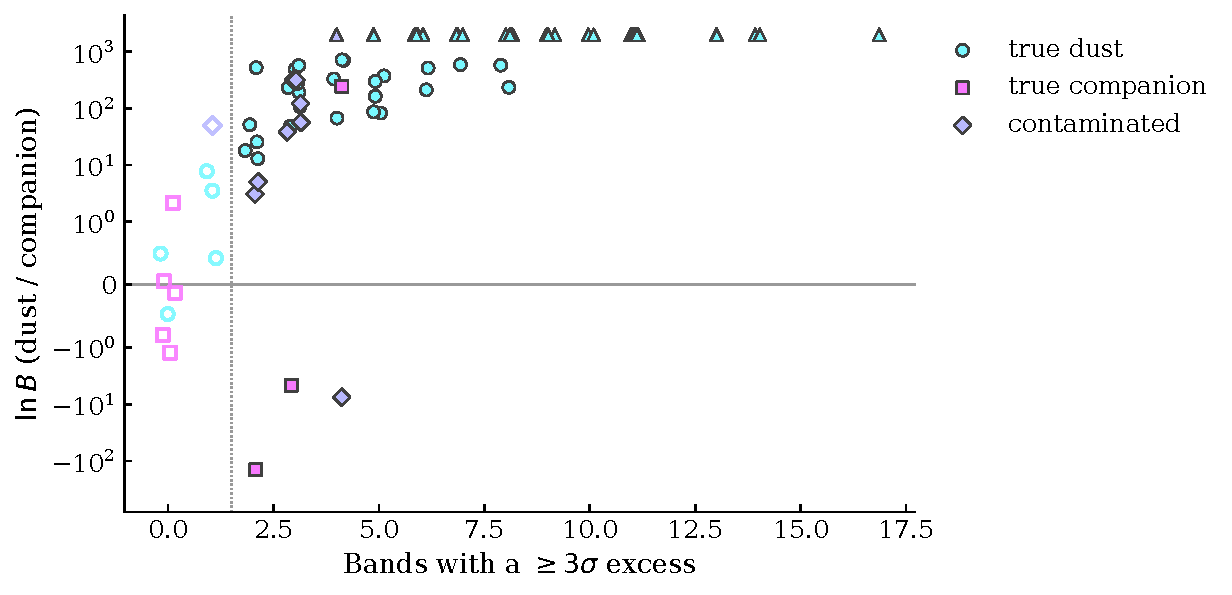
\includegraphics[width=\linewidth]{fig_lnb.pdf}
\caption{Log Bayes factor between the dust and companion hypotheses for the
main-sequence roster, against the number of bands with a $\ge 3\sigma$ excess.
Filled symbols are detected excesses (two or more such bands, right of the dotted
line), open symbols are not. Triangles mark stars for which the losing hypothesis'
evidence underflows to zero. Detected excesses of known origin sit far from zero,
all but \rosDCwrong{} with the sign of their truth; contaminated candidates sit with the dust.}
\label{fig:lnb}
\end{figure}

%%%%%%%%%%%%%%%%%%%%%%%%%%%%%%%%%%%%%%%%%%%%%%%%%%%%%%%%%%%%%%%%%%%%%%%%%%%%%%%
\section{Where archival classification fails}
\label{sec:fail}

If the model comparison is sound wherever an excess is detected, the limits on
archival classification lie elsewhere. We find five.

\paragraph{Sensitivity.} Most injected excesses are not detected
(Table~\ref{tab:inj}). Without a detection the verdict rests largely on the
priors: the roster stars without a detected excess have a median $|\ln B|$ of \rosNondetLnbMed,
and their labels say little about the source. The label is reported, but it is
not a classification (Sect.~\ref{sec:detect}).

\paragraph{Sources outside the hypothesis set.} All four hypotheses place the
excess at the star. Flux from an unrelated source in the beam is therefore
explained by whichever hypothesis fits it best, and for a cold, luminous
background source that is dust. All \contamDet{} of the \citet{theissen2014} candidates
that \citet{silverberg2018} rejected as blends have a detected excess, and all
\contamDisk{} are classified \texttt{disk}, with $\ln B$ from \contamLnbMin{} to \contamLnbMax, and they sit
among the genuine disks in Fig.~\ref{fig:lnb}. The classification is not wrong
about the shape of the excess; it answers a question that assumes the excess
belongs to the star. The same logic runs the other way for 70\,Oph\,A, whose K4
companion 70\,Oph\,B is blended with it in the WISE beam: it is classified
\texttt{companion} ($\ln B = \ophLnb$), which describes the photometry correctly
even though the roster, which expects \texttt{none}, scores it as an error.

\paragraph{Defects in the data.} Evidence ratios amplify systematic errors that a
$\chi^2$ threshold would tolerate. The resolved debris disk TWA\,7 was classified
as a 1.1\,$\Rsun$ companion with $\ln B = -375$ because its IRS short-low
spectrum was a factor 3.6 below the long-low one, placing every band between 5
and $13\,\mu$m some 20$\sigma$ below the photosphere; with the module stitch of
Sect.~\ref{sec:excess} it is a \twaTd\,K disk with
$L_{\rm dust}/L_\star = \twaFd$. The temperature is within the spread of published
single-temperature fits to its far-infrared excess (66--80\,K) and the fractional
luminosity is below theirs ($2.0$--$2.2\times10^{-3}$; \citealt{low2005,riviere2013}). For cool primaries the null and companion hypotheses re-fit the
primary (Sect.~\ref{sec:hyp}) and can absorb such a deficit where the dust
hypotheses cannot, so a data defect there biases the verdict towards them.

\paragraph{A second photosphere.} For hosts cooler than 4000\,K the companion
hypothesis re-fits the primary in every band (Sect.~\ref{sec:hyp}), and its prior
admits a companion as large and nearly as hot as the primary. A weak excess can
then be explained as a second M-dwarf photosphere that shifts the fitted colours,
which the dust hypotheses are not allowed to do. This produces every
misclassified detected injection (\injDetCompGJ{} of the \injDetGJ{} detected disks around
GJ\,876) and one of the \rosDCwrong{} roster misclassifications, GJ\,581
(Sect.~\ref{sec:caveats}).

\paragraph{Probabilities that saturate.} The normalised probabilities of
Eq.~(\ref{eq:probs}) are decision-useful but not calibrated
(Table~\ref{tab:calib}). Two thirds of the main-sequence roster stars receive a
top probability of 1.000 to three decimals, and \relSatWrongPct\% of those are wrong, while
below $p = 0.8$ the probabilities are, if anything, underconfident. The
normalisation discards the
margin by which the winning hypothesis won; the log Bayes factor retains it. We
recommend treating $p$ as a ranking and quoting $\ln B$.

\begin{table}
\caption{Reliability of the reported model probability (main-sequence branch).}
\label{tab:calib}
\centering
%% Generated by cal_run4_analysis/paper_numbers.py. Do not edit by hand.
\begin{tabular}{lrrr}
\toprule
Reported $p$ & $N$ & Mean $p$ & Empirical accuracy \\
\midrule
$[0.00,0.50)$      & 19 & 0.439 & 0.684 \\
$[0.50,0.80)$      & 9 & 0.582 & 0.778 \\
$[0.80,0.9995)$    & 8 & 0.959 & 0.250 \\
$\ge 0.9995$       & 68 & 1.000 & 0.882 \\
\bottomrule
\end{tabular}

\tablefoot{$p$ is the largest of $p_{\rm null}$, $p_{\rm d}$ and $p_{\rm comp}$,
and a star counts as correct when that hypothesis is its true one. The \relN{}
main-sequence stars with a definite classification are used. Mean
overconfidence (mean $p$ minus accuracy) is $\relOverconf$; the three-class Brier score
is \relBrier.}
\end{table}

%%%%%%%%%%%%%%%%%%%%%%%%%%%%%%%%%%%%%%%%%%%%%%%%%%%%%%%%%%%%%%%%%%%%%%%%%%%%%%%
\section{Application: a survey of nearby M dwarfs}
\label{sec:survey}

Peter Pan disks are long-lived accretion disks around M dwarfs of 20--50\,Myr
\citep{silverberg2020}, found through their WISE excesses and confirmed by
accretion signatures and moving-group membership. We asked whether the method
can find new ones in archival photometry alone.

\paragraph{Selection.} From 148\,697 M dwarfs within 125\,pc with a W3 detection,
WISE quality control and an excess screen of $W1-W3 > 1.0$ at $5\sigma$ (the known
Peter Pan disks span $W1-W3 = 1.15$--$2.44$) leave 3695 stars, and a kinematic
youth screen leaves 1372. Of these, \svFrozen{} have frozen photometry and \svOK{} were
fitted successfully; the other \svFewBands{} have too few photometric bands for the
photosphere fit. Two properties of the selection are worth stating on their
own. The standard WISE quality cut \texttt{number\_of\_mates}\,$=0$ removes every
unresolved binary and alone removes four of the seven known Peter Pan disks; and
over-luminosity in the colour--magnitude diagram fails as a youth diagnostic for
this class, because pre-main-sequence brightening and extinction by the disk
cancel.

\paragraph{Result.} An excess is detected in \svDet{} stars, \svDetDisk{} of them are classified
\texttt{disk}, and \svPool{} of those also satisfy the kinematic envelope of the known
systems. \svPoolKnown{} of the six known Peter Pan disks with a parallax are among them,
each decisively a disk ($\ln B \ge \svKnownLnbMin$); the sixth, J0226, has \ppJzzNsig{} significant band. The
method recovers the known systems, and it cannot separate them from the other
\svPoolOther. Their dust temperatures and fractional luminosities are comparable (medians
of \svTdKnown{} and \svTdOther\,K, and $f_{\rm d}$ of $\svFdKnown$ and $\svFdOther$),
which is a selection effect:
$W1-W3 > 1$ admits only $f_{\rm d} \gtrsim 10^{-2}$.

The kinematics say more than the SED. We ran BANYAN~$\Sigma$ \citep{gagne2018}
on Gaia DR3 astrometry \citep{gaia2023} for the \svPool{} stars and, as a control, for
the \banCtlN{} fitted targets without a detected excess inside the same $v_{\rm tan}$
envelope. Both groups passed the same kinematic screen, so a difference between
them reflects the excess rather than the selection. With the 27 associations of
the 2018 models, \banPoolMem{} of the \svPool{} (\banPoolPct\%) are members of a young association with
probability above 0.9, against \banCtlMem{} of the \banCtlN{} controls (\banCtlPct\%); among the \banPoolRvN{} and \banCtlRvN{}
stars with a Gaia radial velocity the fractions are \banPoolRvPct\% and \banCtlRvPct\%. The enrichment
is not an effect of position on the sky: inside the Scorpius--Centaurus region
($280^\circ \le l \le 10^\circ$, $-10^\circ \le b \le 35^\circ$) \banPoolScoPct\% of the
excess stars are members against \banCtlScoPct\% of the controls, and outside it \banPoolOutPct\%
against \banCtlOutPct\%. Most members belong to Lower Centaurus--Crux (\banLCC), Upper
Centaurus--Lupus (\banUCL) and Upper Scorpius (\banUSCO), all of 10--20\,Myr. Of the known
Peter Pan disks, J0446A, J0446B and J0949A are recovered as members of Columba
and Carina ($P = \banPPhiMin$--\banPPhiMax), and J0949B and J0808 at $P \simeq \banPPlo$. With the
larger 2026 model set the fractions rise for both groups, to \banPoolPctTwo\% and \banCtlPctTwo\%, and
the enrichment remains.

The excess-selected sample is therefore substantially young, and published
disk censuses confirm it. Of the \xmMembers{} association members, \xmDiskBearing{} are already
classified as disk-bearing, \xmLtwotwo{} of them in the Sco-Cen census of
\citet{luhman2022b} and the rest in those of Taurus \citep{esplin2019}, the TW Hya
association \citep{luhman2023} and LAMOST M stars \citep{wang2025}, and \xmKnownPP{}
are known Peter Pan disks. \xmDiskless{} are classified by \citet{luhman2022b} as diskless,
although both have a detected disk-like excess here. The remaining \xmNew{} are in no
disk catalogue: \xmNewByGroup, and the rest
in smaller groups. These are candidate new disk hosts.

Accretion is the property that defines a Peter Pan disk, and it is not
photometric, but Gaia XP spectra carry an H$\alpha$ signature from which
\citet{delfini2025} flag accretors. Of the pool, \accN{} stars are so flagged,
including \accKnownPP{} of the \svPoolKnownLow{} known Peter Pan disks in it. Of the \accN, \candA{}
have no catalogued disk and no membership in an association younger than
20\,Myr; \candAnoMem{} of those have no confident membership at all. They are the closest
the archival data come to new Peter Pan disks, and they require spectroscopic
confirmation of accretion and youth (H$\alpha$ line width, lithium), since strong
chromospheric emission in an active M dwarf can mimic an accretion signature at
the resolution of Gaia XP. The SED alone cannot isolate Peter Pan disks; combined
with kinematics and an accretion indicator it reduces 148\,697 M dwarfs to a list
short enough to observe. Both sets of candidates are listed in
Table~\ref{tab:cand}: \candY{} young-association members (the \xmNew{} above and the two
classified as diskless) and \candA{} accretors, \candYA{} of which are also members, \candN{}
stars in all.

None of the survey stars has a Spitzer IRS spectrum, so the IRS stitch of
Sect.~\ref{sec:excess} does not touch this sample.

%%%%%%%%%%%%%%%%%%%%%%%%%%%%%%%%%%%%%%%%%%%%%%%%%%%%%%%%%%%%%%%%%%%%%%%%%%%%%%%
\section{What would resolve the remaining ambiguity}
\label{sec:resolve}

The two remaining ambiguities call for different data.

A blend is a spatial problem, not a spectral one: the contaminant is a separate
source inside the $6\farcs5$ W3 beam, and no additional band at the same
resolution removes it. Archival IRAC and MIPS imaging resolves some cases where it
exists, and deep near-infrared imaging can reveal the background galaxies that
dominate the contamination at faint W3 fluxes \citep{kennedy2012}. The Euclid
Wide Survey reaches $H = 24.4$ (AB, $5\sigma$) over $14\,500\,{\rm deg}^2$
\citep{scaramella2022}, and the Roman high-latitude survey goes deeper still
\citep{rotac2025}, both at sub-arcsecond resolution and far below the
near-infrared counterpart of any source bright enough to produce these W3
excesses (median \svWthreeMed\,mJy). Both avoid the Galactic plane, however, and \svLowBPct\% of
the \svPool{} lie at $|b| < 10^\circ$; only \svHighB{} are at $|b| > 30^\circ$. For the young
Sco-Cen members, which lie close to the plane, targeted imaging remains the
route.

Warm dust around ultracool hosts is a spectral problem. The two hypotheses differ
most between 5 and $8\,\mu$m, where a brown dwarf's spectrum departs from a
blackbody and the dust is still on its Wien side. The only all-sky band there,
AKARI/IRC S9W at $9.2\,\mu$m \citep{ishihara2010}, is too shallow
($\sim$50\,mJy) for these targets, and SPHEREx ends at $4.9\,\mu$m.
\emph{NEO Surveyor} will observe at 4.0--5.2 and $6$--$10\,\mu$m, with a
$5\sigma$ point-source sensitivity of 110--$280\,\mu$Jy per visit in the longer
channel, over ecliptic latitudes $|\beta| \le 40^\circ$ \citep{mainzer2023}. That
is below the faintest W3 flux in our sample (\svWthreeMin\,mJy), so every target inside
its survey zone, \svNeos{} of the \svPool, would be measured in the window where warm dust
and a brown dwarf differ most.

%%%%%%%%%%%%%%%%%%%%%%%%%%%%%%%%%%%%%%%%%%%%%%%%%%%%%%%%%%%%%%%%%%%%%%%%%%%%%%%
\section{Caveats}
\label{sec:caveats}

The white-dwarf branch is not validated here: on the roster it classifies \wdDiskOK{} of
\wdDiskN{} dusty white dwarfs and \wdCompOK{} of \wdCompN{} white dwarfs with brown-dwarf companions
correctly, abstaining on most of the rest (Table~\ref{tab:bycat}). \texttt{fit\_binary} requires an externally supplied flux ratio
and characterises a companion rather than detecting one. The injection hosts carry
more bands than the survey stars, so injection performance does not transfer to
the survey directly. The classification also depends on where the photosphere
fit ends (Sect.~\ref{sec:routing}).

\paragraph{The photospheric baseline in the mid-infrared.} \citet{stefanov2026}
find \ariadne{} temperatures $330 \pm 55$\,K cooler than those of SPOG+, a fit of
PARSEC tracks to $J$, $K_s$ and the parallax, for main-sequence stars below about
4500\,K. The comparison is between two methods, neither anchored to an
independent temperature scale. What matters here is the mid-infrared photosphere
against which the excess is measured, and we measured it directly. For 246 field
dwarfs within 50\,pc without a detected excess, all fainter than $W3 = 5$ and
hence clear of saturation, the median of $(F^{\rm obs} - F^\star)/F^\star$ is
$-3\%$ at W3 for FGK stars, within the absolute calibration of WISE
\citep{wright2010,jarrett2011}, but $-9.1 \pm 0.4\%$ at 3000--3500\,K and
$-12.3 \pm 0.7\%$ at 3500--4000\,K, with $-6.5$ and $-8.4\%$ at W2; W4 is too noisy
to show a trend. The photosphere over-predicts the mid-infrared flux of M dwarfs
by about 10\%. It is not a zero-point effect: the Vega zero points used by
\ariadne{} reproduce those of \citet{jarrett2011} to 0.8\% at W3 and 1.9\% at W4.
Its size is what a 330\,K too cool photosphere produces once rescaled to the
near-infrared (10--15\% at W3 and W4 in BT-Settl), and it has the sign of the
negative cool-star W3/W4 residuals of \citet{cotten2016}. Brighter stars add a
saturation term: the clean nulls of the roster, most of them brighter than
$W3 = 4$, show deficits several per cent larger.

Left uncorrected, the bias lowers M-dwarf excesses rather than creating them, so
it costs sensitivity to weak mid-infrared excesses; it does not touch the
separation of dust from companions, which is decided at $|\ln B| \gg 1$. We
correct it empirically (Sect.~\ref{sec:excess}).

\paragraph{Two failure modes of the cool-host branch.} The joint fit lets a
companion contribute to the optical and near-infrared bands, as it physically
does; when the single grid gets a bright M dwarf's colours wrong, a companion can
absorb the mismatch. Gliese\,1, with no significant excess band, is
classified \texttt{companion} for this reason, the companion being a
\glOneTtwo\,K, \glOneRtwo\,$\Rsun$ second photosphere beside a \glOneTeff\,K primary. With a
weak excess the same freedom decides the class: the debris disk of GJ\,581, detected
in \gjFiveNsig{} bands, is classified \texttt{companion}, and so are \injDetCompGJ{} of the \injDetGJ{}
detected injected disks around GJ\,876 (Sect.~\ref{sec:separate}). Separately, a photosphere fit that
is bimodal in $T_{\rm eff}$ propagates directly into the verdict: WISE\,J1002+0741
converges either to 3670\,K and $0.06\,\Rsun$ or to 2410\,K and $0.39\,\Rsun$, and
its classification follows, decisively in either direction. A verdict is only as
stable as the photosphere fit beneath it.

%%%%%%%%%%%%%%%%%%%%%%%%%%%%%%%%%%%%%%%%%%%%%%%%%%%%%%%%%%%%%%%%%%%%%%%%%%%%%%%
\section{Summary}
\label{sec:summary}

We have added to \ariadne{} a Bayesian comparison of four hypotheses for an
infrared excess, computed on the bands that every atmosphere grid in the ensemble
reaches and against the model-averaged photosphere, and we have measured where it
can be trusted.

\begin{enumerate}
  \item Once an excess is detected, dust and companions separate. On the
        literature roster \rosDCok{} of \rosDC{} detected excesses of known origin receive
        their true class, decisively; among the injections, \injDiskAsCompDet{} of \injDiskDet{}
        detected disks are taken for companions, all around one M4 host, and
        none of \injCompDet{} detected companions for disks.
  \item The separation is physical. A companion bounded by its primary's radius
        and temperature cannot supply a cold, luminous excess, and substellar
        companions are detectable only around faint hosts. The degeneracy
        survives only for dust of about \injVBwarmT\,K around the M8 host, where the
        classifier abstains.
  \item What limits archival classification is sensitivity, flux that does not
        belong to the star, a second photosphere that the cool-host joint fit
        can substitute for a weak excess, and data defects. The method detects
        \injDiskFlagPctInt\% of injected
        disks and \injCompFlagPct\% of injected companions; contaminated M-dwarf candidates are
        classified as dust as decisively as real disks; and a single mis-pointed
        IRS spectrum turned a resolved debris disk into a stellar-sized companion
        until the spectrum was repaired.
  \item The normalised probabilities saturate and should be read as a ranking;
        the log Bayes factor keeps the information they discard.
  \item Among 1372 nearby M dwarfs the known Peter Pan disks are recovered as
        disks, together with \svPoolOther{} other stars the SED cannot distinguish from
        them. Their kinematics can: \banPoolPct\% are members of young associations,
        \banRatio{} times the rate among matched stars without an excess, most of them
        in Sco-Cen. An archival SED search cannot single out Peter Pan disks,
        but it does isolate young M dwarfs with disk-like excesses.
\end{enumerate}

\begin{acknowledgements}
\todo{funding statement.}
This work has made use of data from the European Space Agency (ESA) mission
{\it Gaia} (\url{https://www.cosmos.esa.int/gaia}), processed by the {\it Gaia}
Data Processing and Analysis Consortium (DPAC,
\url{https://www.cosmos.esa.int/web/gaia/dpac/consortium}). Funding for the DPAC
has been provided by national institutions, in particular the institutions
participating in the {\it Gaia} Multilateral Agreement
\citep{gaiacollaboration2016,gaia2023}.
This publication makes use of data products from the Two Micron All Sky Survey
\citep{skrutskie2006}, which is a joint project of the University of
Massachusetts and the Infrared Processing and Analysis Center/California
Institute of Technology, funded by the National Aeronautics and Space
Administration and the National Science Foundation.
This publication makes use of data products from the Wide-field Infrared Survey
Explorer \citep{wright2010}, which is a joint project of the University of
California, Los Angeles, and the Jet Propulsion Laboratory/California Institute
of Technology, and NEOWISE \citep{mainzer2011}, which is a project of the Jet
Propulsion Laboratory/California Institute of Technology. WISE and NEOWISE are
funded by the National Aeronautics and Space Administration. We use the AllWISE
and CatWISE2020 \citep{marocco2021} catalogues.
This work is based in part on observations made with the Spitzer Space Telescope
\citep{werner2004}, with IRAC \citep{fazio2004}, IRS \citep{houck2004} and MIPS
\citep{rieke2004}, which was operated by the Jet Propulsion Laboratory,
California Institute of Technology under a contract with NASA.
\todo{GLIMPSE catalogue reference (VizieR II/293).}
\todo{CASSIS acknowledgement: copy the requested text from cassis.sirtf.com
(the site blocks scripted access).}
This work uses PACS \citep{poglitsch2010} and SPIRE \citep{griffin2010}
photometry from {\it Herschel} \citep{pilbratt2010}.
This research is based on observations with AKARI \citep{murakami2007}, a JAXA
project with the participation of ESA \citep{ishihara2010,doi2015}.
This research is based on observations made with the Galaxy Evolution Explorer
(GALEX).
Funding for SDSS-III has been provided by the Alfred P. Sloan Foundation, the
Participating Institutions, the National Science Foundation, and the U.S.
Department of Energy Office of Science. The SDSS-III web site is
\url{http://www.sdss3.org/}. SDSS-III is managed by the Astrophysical Research
Consortium for the Participating Institutions of the SDSS-III Collaboration
including the University of Arizona, the Brazilian Participation Group,
Brookhaven National Laboratory, Carnegie Mellon University, University of
Florida, the French Participation Group, the German Participation Group, Harvard
University, the Instituto de Astrofisica de Canarias, the Michigan State/Notre
Dame/JINA Participation Group, Johns Hopkins University, Lawrence Berkeley
National Laboratory, Max Planck Institute for Astrophysics, Max Planck Institute
for Extraterrestrial Physics, New Mexico State University, New York University,
Ohio State University, Pennsylvania State University, University of Portsmouth,
Princeton University, the Spanish Participation Group, University of Tokyo,
University of Utah, Vanderbilt University, University of Virginia, University of
Washington, and Yale University.
The Pan-STARRS1 Surveys (PS1) and the PS1 public science archive
\citep{flewelling2020} have been made possible through contributions by the
Institute for Astronomy, the University of Hawaii, the Pan-STARRS Project
Office, the Max-Planck Society and its participating institutes, the Max Planck
Institute for Astronomy, Heidelberg and the Max Planck Institute for
Extraterrestrial Physics, Garching, The Johns Hopkins University, Durham
University, the University of Edinburgh, the Queen's University Belfast, the
Harvard-Smithsonian Center for Astrophysics, the Las Cumbres Observatory Global
Telescope Network Incorporated, the National Central University of Taiwan, the
Space Telescope Science Institute, the National Aeronautics and Space
Administration under Grant No. NNX08AR22G issued through the Planetary Science
Division of the NASA Science Mission Directorate, the National Science
Foundation Grant No. AST-1238877, the University of Maryland, Eotvos Lorand
University (ELTE), the Los Alamos National Laboratory, and the Gordon and Betty
Moore Foundation.
The national facility capability for SkyMapper has been funded through ARC LIEF
grant LE130100104 from the Australian Research Council, awarded to the
University of Sydney, the Australian National University, Swinburne University
of Technology, the University of Queensland, the University of Western
Australia, the University of Melbourne, Curtin University of Technology, Monash
University and the Australian Astronomical Observatory. SkyMapper is owned and
operated by The Australian National University's Research School of Astronomy
and Astrophysics. The survey data were processed and provided by the SkyMapper
Team at ANU. The SkyMapper node of the All-Sky Virtual Observatory (ASVO) is
hosted at the National Computational Infrastructure (NCI). Development and
support of the SkyMapper node of the ASVO has been funded in part by Astronomy
Australia Limited (AAL) and the Australian Government through the
Commonwealth's Education Investment Fund (EIF) and National Collaborative
Research Infrastructure Strategy (NCRIS), particularly the National eResearch
Collaboration Tools and Resources (NeCTAR) and the Australian National Data
Service Projects (ANDS). We use SkyMapper DR4 \citep[][doi:10.25914/5M47-S621]{onken2024}.
\todo{APASS acknowledgement: copy from archive.aavso.org/apass (blocked to
scripted access); DR9 is the release used.}
This research has made use of the NASA/IPAC Infrared Science Archive, which is
funded by the National Aeronautics and Space Administration and operated by the
California Institute of Technology.
This research has made use of the SIMBAD database \citep{wenger2000}, CDS,
Strasbourg Astronomical Observatory, France, and of the VizieR catalogue access
tool \citep{ochsenbein2000}, CDS, Strasbourg Astronomical Observatory, France
(DOI: 10.26093/cds/vizier).
This research has made use of the SVO Filter Profile Service ``Carlos Rodrigo''
\citep{rodrigo2024}, funded by MCIN/AEI/10.13039/501100011033/ through grant
PID2023-146210NB-I00.
This research has made use of NASA's Astrophysics Data System Bibliographic
Services.
We used \texttt{numpy} \citep{harris2020}, \texttt{scipy} \citep{virtanen2020},
\texttt{astropy} \citep{astropy2013,astropy2018,astropy2022},
\texttt{astroquery} \citep{ginsburg2019}, \texttt{matplotlib}
\citep{hunter2007}, \texttt{dynesty} \citep{speagle2020} and BANYAN~$\Sigma$
\citep{gagne2018}.
\end{acknowledgements}

\bibliographystyle{aa}
\bibliography{ariadne2}

\begin{appendix}
\onecolumn
\section{New disk candidates}
\label{app:cand}
Table~\ref{tab:cand} lists the survey stars with a detected disk-like excess and
no disk in a published census that are either members of a young
association or flagged as accretors by Gaia XP (Sect.~\ref{sec:survey}). It is
also available in machine-readable form.
\begin{longtable}{lrrlrlcrrr}
\caption{New disk candidates from the M-dwarf survey (Sect.~\ref{sec:survey}). Flags: Y, member of a young association with $P > 0.9$ (BANYAN~$\Sigma$, 2018 models); A, Gaia XP accretion signature \citep{delfini2025} and no membership in an association younger than 20\,Myr. No star is classified as disk-bearing in a published census; the two marked $^\dagger$ are classified as diskless (Class III) by \citet{luhman2022b}. $T_{\rm d}$ and $f_{\rm d}$ are the single-temperature dust fit; $\ln B$ is dust over companion; uf, the companion evidence underflows in double precision.}\label{tab:cand}\\
\toprule
Gaia DR3 & $d$ (pc) & $T_{\rm eff}$ (K) & Group & $P$ & Flags & $n_{\rm sig}$ & $\ln B$ & $T_{\rm d}$ (K) & $f_{\rm d}$ \\
\midrule
\endfirsthead
\toprule
Gaia DR3 & $d$ (pc) & $T_{\rm eff}$ (K) & Group & $P$ & Flags & $n_{\rm sig}$ & $\ln B$ & $T_{\rm d}$ (K) & $f_{\rm d}$ \\
\midrule
\endhead
\bottomrule
\endfoot
5568864873853123456 & 82.6 & 2842 & Col & 0.93 & YA & 3 & 89 & 234 & $0.056$ \\
4860968432844716544 & 102.1 & 2400 & $\chi^1$\,For & 1.00 & YA & 3 & 75 & 444 & $0.072$ \\
4854879573671981056 & 104.4 & 2754 & $\chi^1$\,For & 1.00 & YA & 2 & 79 & 256 & $0.032$ \\
4854506946605939712 & 106.8 & 2873 & $\chi^1$\,For & 0.91 & YA & 3 & 87 & 467 & $0.072$ \\
3403529658143595392 & 107.0 & 2932 & 118\,Tau & 0.98 & Y & 3 & 57 & 463 & $0.043$ \\
5224035654899133440 & 73.0 & 2314 & Car & 1.00 & Y & 2 & 27 & 361 & $0.097$ \\
5199797749993133440 & 96.4 & 3303 & $\epsilon$\,Cha & 0.94 & Y & 6 & 243 & 151 & $0.085$ \\
5788500121160692480 & 100.4 & 2249 & $\epsilon$\,Cha & 0.98 & Y & 3 & 38 & 371 & $0.082$ \\
5788551695132821376 & 101.6 & 2689 & $\epsilon$\,Cha & 1.00 & Y & 3 & 139 & 416 & $0.086$ \\
5788622854149598336 & 102.2 & 2946 & $\epsilon$\,Cha & 1.00 & Y & 4 & uf & 251 & $0.035$ \\
5788625396770225152 & 102.8 & 2866 & $\epsilon$\,Cha & 1.00 & Y & 4 & uf & 239 & $0.044$ \\
5869105181216442240 & 92.4 & 2896 & LCC & 0.99 & Y & 2 & 12 & 207 & $0.015$ \\
5870670988861993216 & 92.4 & 3291 & LCC & 0.98 & Y & 3 & 46 & 305 & $0.009$ \\
6126460514883217920 & 95.5 & 2752 & LCC & 0.95 & Y & 3 & 22 & 397 & $0.097$ \\
5844015768940264320 & 96.6 & 2811 & LCC & 0.95 & Y & 3 & 148 & 219 & $0.068$ \\
6071792178303014912 & 98.2 & 3653 & LCC & 1.00 & Y & 3 & 98 & 169 & $0.027$ \\
5336913343986807040 & 102.5 & 3121 & LCC & 0.97 & Y & 2 & 38 & 164 & $0.032$ \\
5346463427106534784 & 102.8 & 2716 & LCC & 0.97 & Y & 3 & 54 & 505 & $0.064$ \\
5336376503118529536 & 102.8 & 3008 & LCC & 1.00 & Y & 3 & 57 & 243 & $0.021$ \\
5843724192198636416 & 103.1 & 3040 & LCC & 0.98 & Y & 3 & 64 & 555 & $0.047$ \\
5344945860538454272 & 104.9 & 3091 & LCC & 0.95 & Y & 2 & 68 & 377 & $0.017$ \\
5341805449189956992$^\dagger$ & 106.7 & 2808 & LCC & 1.00 & Y & 2 & 32 & 203 & $0.035$ \\
5338341369096585728 & 112.5 & 3148 & LCC & 0.99 & Y & 2 & 69 & 187 & $0.053$ \\
6056102387871359488$^\dagger$ & 114.2 & 2862 & LCC & 1.00 & Y & 3 & 53 & 334 & $0.039$ \\
6124958749509664640 & 114.5 & 2346 & LCC & 1.00 & Y & 2 & 53 & 323 & $0.039$ \\
6057314187161287424 & 114.6 & 3152 & LCC & 1.00 & Y & 3 & 74 & 520 & $0.042$ \\
5337072223425732608 & 117.5 & 2946 & LCC & 0.99 & Y & 2 & 56 & 239 & $0.099$ \\
5234567400053584640 & 118.7 & 2931 & LCC & 0.97 & Y & 3 & 71 & 411 & $0.062$ \\
147546080967742720 & 114.5 & 2914 & Tau & 1.00 & Y & 4 & 353 & 223 & $0.044$ \\
3241254244532020608 & 100.1 & 2646 & 32\,Ori & 0.98 & Y & 3 & 36 & 494 & $0.081$ \\
6090811289904309504 & 104.0 & 2618 & UCL & 1.00 & Y & 3 & 113 & 451 & $0.071$ \\
6029907137521434752 & 106.1 & 3452 & UCL & 0.92 & Y & 3 & 148 & 174 & $0.099$ \\
6005726304142187264 & 107.5 & 2592 & UCL & 1.00 & Y & 2 & 31 & 455 & $0.044$ \\
6010284570110648576 & 124.9 & 2953 & UCL & 0.99 & Y & 3 & 34 & 489 & $0.099$ \\
6243943882070642176 & 105.5 & 3152 & USco & 0.97 & Y & 2 & 25 & 149 & $0.048$ \\
6243457550035199744 & 106.7 & 3011 & USco & 0.99 & Y & 3 & 35 & 224 & $0.016$ \\
6236850176648443264 & 115.7 & 2055 & USco & 0.99 & Y & 2 & 45 & 195 & $0.098$ \\
6049313522040863616 & 119.0 & 2909 & USco & 0.98 & Y & 2 & 52 & 170 & $0.047$ \\
6046081778190577920 & 119.4 & 3106 & USco & 0.98 & Y & 6 & uf & 219 & $0.020$ \\
6051770346414064896 & 120.3 & 2949 & USco & 0.99 & Y & 4 & uf & 158 & $0.038$ \\
6237639862214679680 & 123.6 & 3163 & USco & 0.95 & Y & 3 & 5.5 & 478 & $0.096$ \\
5047057271152602240 & 100.6 & 2748 & $\chi^1$\,For & 0.99 & Y & 3 & 71 & 241 & $0.064$ \\
4854879577968187392 & 101.1 & 2894 & $\chi^1$\,For & 1.00 & Y & 2 & 79 & 262 & $0.038$ \\
6044879015558339072 & 38.5 & 2766 & -- & -- & A & 3 & 99 & 498 & $0.065$ \\
6886178038419703168 & 62.3 & 2976 & -- & -- & A & 3 & 177 & 247 & $0.046$ \\
2064379058776701824 & 66.0 & 2920 & -- & -- & A & 2 & 35 & 156 & $0.030$ \\
6065042242049473792 & 72.8 & 2973 & -- & -- & A & 3 & 108 & 520 & $0.069$ \\
4655994623337799808 & 82.3 & 2695 & -- & -- & A & 7 & 650 & 290 & $0.071$ \\
3308700559817832064 & 83.9 & 2970 & -- & -- & A & 2 & 194 & 222 & $0.060$ \\
3290126127637212672 & 87.4 & 2726 & -- & -- & A & 2 & 88 & 473 & $0.098$ \\
6237002699525087488 & 87.9 & 2759 & -- & -- & A & 2 & 16 & 157 & $0.029$ \\
21174364863552000 & 89.9 & 2950 & -- & -- & A & 3 & 36 & 412 & $0.038$ \\
3012231508679235072 & 91.1 & 3101 & -- & -- & A & 4 & 474 & 264 & $0.035$ \\
5280226578890455168 & 93.0 & 3036 & -- & -- & A & 2 & 164 & 263 & $0.036$ \\
5199332484776169600 & 95.4 & 2822 & -- & -- & A & 4 & uf & 222 & $0.030$ \\
5222404361896063232 & 97.8 & 2968 & -- & -- & A & 2 & 150 & 242 & $0.045$ \\
5209140815689766144 & 99.6 & 2836 & -- & -- & A & 5 & uf & 238 & $0.050$ \\
4767548770987942272 & 100.3 & 3216 & -- & -- & A & 3 & 70 & 490 & $0.064$ \\
3401712332924254848 & 104.4 & 2743 & -- & -- & A & 3 & 44 & 466 & $0.047$ \\
2204844001395769600 & 106.5 & 2987 & -- & -- & A & 2 & 11 & 176 & $0.036$ \\
1354342212226832768 & 107.8 & 2781 & -- & -- & A & 2 & 61 & 277 & $0.049$ \\
5060663418310359424 & 112.5 & 2941 & -- & -- & A & 3 & 89 & 184 & $0.050$ \\
3215746438056812288 & 114.5 & 2853 & -- & -- & A & 2 & 14 & 196 & $0.037$ \\
6316503952920196608 & 114.8 & 2905 & -- & -- & A & 3 & 84 & 472 & $0.061$ \\
5081640790199917696 & 116.7 & 2864 & -- & -- & A & 2 & 119 & 213 & $0.092$ \\
4639274109494255232 & 119.2 & 2785 & -- & -- & A & 3 & 62 & 500 & $0.062$ \\
\end{longtable}

\end{appendix}

\end{document}
